


\begin{FraseCelebre}
\begin{Frase}
%Si quieres ser le�do m�s de una vez, no vaciles en borrar a menudo.
%Rem tene, verba sequentur (Si dominas el tema, las palabras vendr�n solas)
\end{Frase}
\begin{Fuente}
%Horacio
%Cat�n el Viejo
\end{Fuente}
\end{FraseCelebre}


\chapter{Especificaci\'on del protocolo de comunicaci\'on}
\label{cap3}
\label{cap:especificacion}


La finalidad de este trabajo es conseguir la conexi\'on entre 2 dispositivos con la creaci\'on de una librer\'ia para un motor de videojuegos. Uno de ellos va funcionar como un controlador de videojuegos y otro como ejecutor del juego. Para que esta comunicaci\'on se consiga es necesario analizar y definir las funcionalidades que se quieren ofrecer a los desarrolladores que usen la librer\'ia. \\

En este cap\'itulo se va realizar un an\'alisis de las diferentes funcionalidades que son necesarias para que la comunicaci\'on pueda realizarse. Se expondr\'an las ventajas y las desventajas de cada una de estas funcionalidades y por \'ultimo se definir\'a el protocolo de comunicaci\'on entre los 2 dispositivos involucrados en este trabajo.


%-------------------------------------------------------------------
\section{Arquitectura del proyecto a alto nivel}
%-------------------------------------------------------------------

\begin{figure}[!htb]
    \centering
    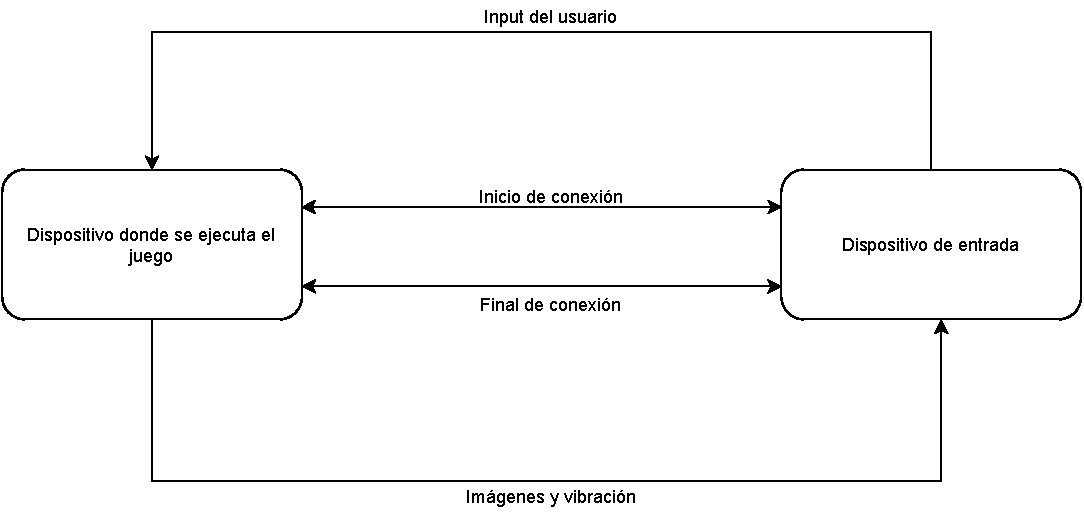
\includegraphics[width=0.90\textwidth]{./Imagenes/Vectorial/Diagrama protocolo.pdf}
    \caption{Esquema de comunicaci\'on del proyecto}
\label{Fig:arquitectura}
\end{figure}

Como ya hemos mencionado, el objetivo a alto nivel se explica en la figura~\ref{Fig:arquitectura}. 

Para conseguir usar el dispositivo m\'ovil como mando para videojuegos se plantearon las posibles caracter\'isticas que podr\'ian incluirse. Como se detalla m\'as adelante, estas opciones difieren en la versatilidad que se le ofrece al usuario de la librer\'ia, la complejidad de programaci\'on y el ancho de banda usado durante la ejecuci\'on del juego. \\

La primera de estas opciones se basa en el uso de im\'agenes est\'aticas de mandos cargados previamente en la aplicaci\'on del m\'ovil. La comunicaci\'on entonces ser\'ian las pulsaciones que se env\'ian desde el m\'ovil al ordenador.  En este esquema el feedback viene dado por la aplicaci\'on que se ejecuta en el dispositivo m\'ovil. La principal ventaja en el env\'io de una \'unica imagen est\'atica es el poco uso de ancho de banda. La \'unica comunicaci\'on que se tiene por red es el env\'io de las pulsaciones del usuario en la pantalla del m\'ovil al ordenador. Esta comunicaci\'on puede realizarse utilizando TCP y conseguir as\'i que no se pierda ninguna pulsaci\'on del usuario. Otra ventaja que ofrece es la poca complejidad que supone para el usuario final de la librer\'ia. Con este sistema, el juego ser\'ia notificado de la llegada de pulsaciones desde el tel\'efono gracias a la librer\'ia desarrollada. El desarrollador del juego \'unicamente tendr\'ia que encargarse de decidir qu\'e hacer con la llegada de cada pulsaci\'on. Esto lleva directamente a la primera desventaja, la poca versatilidad que se le da al usuario de la librer\'ia. Al no haber una comunicaci\'on desde el videojuego hasta el m\'ovil, perdemos la oportunidad de que el desarrollador del juego modifique el mando que quiere utilizar o que ordene al tel\'efono activar la vibraci\'on a su gusto.\\

Para resolver el problema de la modificaci\'on del mando que usar se plante\'o una nueva caracter\'istica: permitir que el juego env\'ie im\'agenes en formato .PNG a lo largo de la sesi\'on de juego. Para que esto sea posible se tiene que habilitar el env\'io de datos en ambas direcciones. Hacer esto supone un aumento en el uso necesario del ancho de banda a cambio de dar m\'as versatilidad al usuario de la librer\'ia. Para conseguir la modificaci\'on de las im\'agenes, Android ofrece un sistema de capas en las im\'agenes que se describan en el archivo de manifiesto. Estas capas se pintan en orden descendiente, siendo la \'ultima im\'agen declarada la que tapar\'ia al resto. \\

Para disminuir el impacto en el ancho de banda se plante\'o la opci\'on de que el env\'io del mando desde el juego al dispositivo m\'ovil se hiciese \'unicamente al inicio de la conexi\'on. Hacerlo de esta manera permitir\'ia al usuario de la librer\'ia modificar el mando con el que se quiere jugar pero este no se podr\'ia cambiar en ning\'un momento de la ejecuci\'on. Esta decisi\'on aumenta el coste en el ancho de banda al inicio de la conexi\'on pero disminuye dr\'asticamente una vez que la imagen del mando ha sido guardada, lo que permite seguir usando TCP como protocolo de transmisi\'on.\\


Otra nueva caracter\'istica da la posibilidad al usuario de la librer\'ia de enviar streaming de video al dispositivo m\'ovil y que este lo muestre por pantalla. Para que esto sea posible la comunicaci\'on entre ambos dispositivos tiene que realizarse en ambos sentidos durante toda la ejecuci\'on con un intercambio constante de datos. Como esta caracter\'isitica es la m\'as vers\'atil para el usuario de la librer\'ia, en esta arquitectura se dar\'ia la posibilidad de controlar la vibraci\'on tambi\'en al desarrollador. Darle todas estas caracter\'isticas al desarrollador implica un aumento en la complejidad del c\'odigo que este tiene que implementar. Dado que el consumo del ancho de banda sube de manera considerable, en este dise\~no se ha optado por modificar el protocolo de transmisi\'on de TCP a UDP para disminuir el consumo. Esta caracter\'istica es m\'as vers\'atil para el desarrollador del videojuego pero tambi\'en es m\'as costosa en cuanto al ancho de banda que usa. Esto implica que se asume una posible p\'erdida de pulsaciones realizadas por el usuario o una posible p\'erdida de frames en el env\'io del streaming de video.\\

Este \'ultimo conjunto de caracter\'isticas ha sido el utilizado para este proyecto. Las funcionalidades que se ofrecen al usuario de la librer\'ia son:

\begin {itemize}
\item Env\'io de pulsaciones desde el dispositivo m\'ovil al juego.
\item Env\'io de streaming de im\'agenes en formato .PNG desde el juego al m\'ovil.
\item Env\'io de orden de vibraci\'on del juego al m\'ovil.
\end {itemize}

Para que el desarrollador tenga un control total de lo que se env\'ia en cada momento, se da la opci\'on de enviar un mensaje de vibraci\'on al dispositivo m\'ovil. Esto permite que el m\'ovil vibre no solo por las pulsaciones, sino, por ejemplo, cuando el jugador reciba da\~no o se choque si est\'a jugando a un juego de conducci\'on. En la siguiente secci\'on se detalla el protocolo desarrollado y en el pr\'oximo cap\'itulo se detallar\'a la implementaci\'on de la parte de m\'ovil y PC.


%-------------------------------------------------------------------
\section{Protocolo de comunicaci\'on entre juego y dispositivo de entrada}
%-------------------------------------------------------------------

Un protocolo de comunicaci\'on es un sistema de reglas que permiten a 2 o m\'as dispositivos comunicarse entre ellos. Estas reglas se establecen para permitir la transmisi\'on de datos y la forma en la que la informaci\'on debe ser procesada. Cada mensaje tiene un significado exacto destinado a obtener una respuesta de un rango de posibles respuestas predeterminadas para esa situaci\'on en particular. Una de las caracter\'isticas principales de un protocolo de comunicaci\'on es que ambas partes tienen que conocer y usar los mensajes que se van a enviar y a recibir. \\

La estructura de estos mensajes consta de 2 partes: el primer byte define el tipo del mensaje y en los bytes posteriores viene la informaci\'on esperada. Con esto se consigue tener un tama\~no de datagrama diferente dependiendo de la informaci\'on que requiera mensaje. Adem\'as, es ampliable en caso de querer definir mensajes nuevos ya que no se utilizan todos los valores de este primer byte. En los siguientes p\'arrafos se van a describir cada uno de los mensajes que est\'an definidos para este protocolo. \\

El byte de cabecera indica el tipo de mensaje y la informaci\'on que se espera. En esta primera versi\'on del protocolo se han utilizado los 7 primeros valores. Existen 2 mensajes que no tienen cabecera, el primer mensaje que realiza la conexi\'on y el env\'io de la resoluci\'on del dispositivo m\'ovil. Para que la conexi\'on se realice con \'exito, el dispositivo de entrada debe enviar la versi\'on del protocolo en la que se encuentra. En caso de que la versi\'on coincida en ambos dispositivos, la conexi\'on se dar\'a por buena. Tras el env\'io de la versi\'on del protocolo, el dispositivo m\'ovil enviar\'a su resoluci\'on para (tabla~\ref{table:1}). En caso contrario, el mensaje es descartado ya que contestar a este mensaje puede ser una brecha de seguridad. Al utilizar UDP, contestar a mensajes de conexi\'on fallidos puede desembocar en un ataque similar a una inundaci\'on UDP, \cite{udpflood}.\\


\begin{table}[h!]
\centering
\begin{tabular}{|c|c|} 
\hline
0-15                   & 16-32                   \\
\hline
 \multicolumn{1}{|c|}{Ancho} & \multicolumn{1}{c|}{Alto}  \\
\hline
\end{tabular}
\caption{Env\'io de la resoluci\'on del m\'ovil al juego.}
\label{table:1}
\end{table}

Una vez los 2 primeros mensajes son enviados, los siguientes se enviar\'an de forma as\'incrona y se diferencian por el primer byte del datagrama. Este primer byte tiene como funci\'on ser usado como cabecera y poder diferenciar cada tipo de mensaje. Los posibles mensajes son:\\

\begin {itemize}
\item El valor de cabecera 0 es utilizado para los mensajes de tipo pulsacion. Estos mensajes son enviados desde el dispositivo m\'ovil (tabla~\ref{table:2}).
\item  El valor de cabecera 1 es utilizado para los mensajes de tipo \textit{tracker}. 
\item  El valor de cabecera 2 es utilizado para avisar al dispositivo m\'ovil de activar la vibraci\'on durante un tiempo establecido.
\item  El valor de cabecera 3 es utilizado para enviar im\'agenes comprimidas desde el juego al m\'ovil.
\item  El valor de cabecera 4 es utilizado para avisar sobre el cierre de conexi\'on por parte del dispositivo que lo env\'ia.
\item  El valor de cabecera 5 es utilizado para establecer el tiempo de vibraci\'on en caso de que este se active (tabla~\ref{table:3}).
\item  El valor de cabecera 6 es utilizado para los mensajes \textit{keep alive}, utilizados para comprobar que la conexi\'on sigue activa en caso de que el usuario no realice pulsaciones en un tiempo determinado.
\end {itemize}

%----------------------------------------------------------------------------------------------------------

\begin{table}[h!]
\centering
\begin{tabular}{|c|c|c|c|} 
\hline
Byte de cabecera                   & 8-15                            & 16-31 & 32-47 \\ 
\hline
\multicolumn{1}{|c|}{00000000} & Tipo de pulsaci\'on & \multicolumn{1}{c|}{Posici\'on X} & \multicolumn{1}{c|}{Posici\'on Y}  \\
\hline
\end{tabular}
\caption{Pulsaci\'on enviada desde el dispositivo m\'ovil al ejecutor del juego}
\label{table:2}
\end{table}

%----------------------------------------------------------------------------------------------------------

\begin{table}[h!]
\centering
\begin{tabular}{|c|c|} 
\hline
Byte de cabecera                                     & 8-23                   \\
\hline
\multicolumn{1}{|c|}{00000101} & \multicolumn{1}{c|}{Tiempo de vibraci\'on}  \\
\hline
\end{tabular}
\caption{Tiempo de vibraci\'on del dispositivo m\'ovil en milisegundos}
\label{table:3}
\end{table}

%----------------------------------------------------------------------------------------------------------

Los mensajes de los que no se ha puesto ninguna tabla es porque son utilizados para avisar de eventos, por lo que con la cabecera es suficiente. El tiempo de vibraci\'on del dispositivo puede modificarse en cualquier momento para que el usuario de la librer\'ia pueda modificarla en funci\'on del momento del juego. En la figura~\ref{Fig:protocolo} se puede observar el flujo de datagramas durante una ejecuci\'on del juego.\\

\begin{figure}[h]

\centering
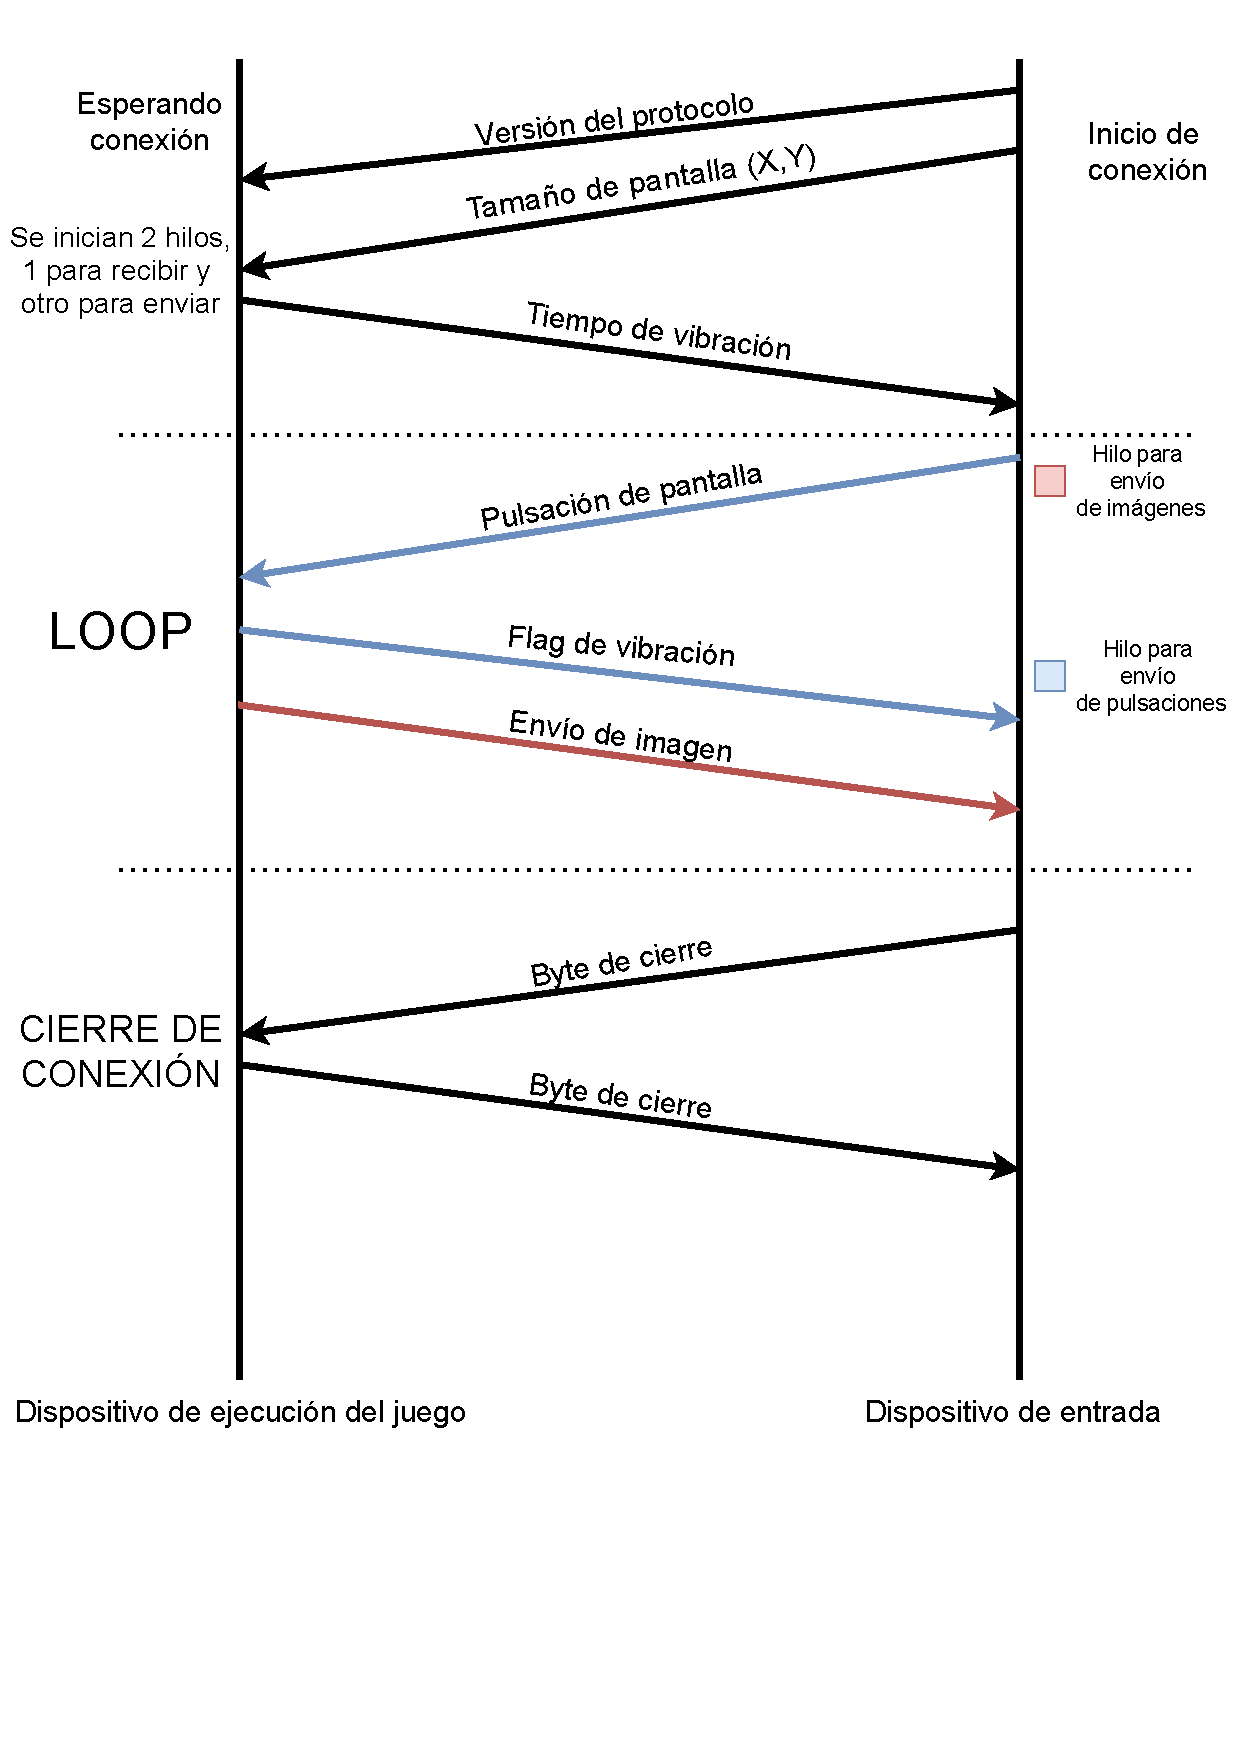
\includegraphics[width=0.7\textwidth]{./Imagenes/Vectorial/Arquitectura}
\caption{Diagrama del protocolo de comunicaci\'on entre ambos dispositivos}
\label{Fig:protocolo}
\end{figure}

Las im\'agenes enviadas est\'an comprimidas en formato PNG. El tama\~no de esta im\'agen puede variar en funci\'on de la complejidad de la im\'agen. En pruebas realizadas, esta im\'agen pesa aproximadamente 24KB, un valor bastante inferior a los 64KB que admite UDP como tama\~no m\'aximo de paquete. En este protocolo no se ha tenido en cuenta la divisi\'on de datagramas por superar el tama\~no m\'aximo soportado por UDP.\\

\vspace{30mm}

\bigskip
\Large{\textbf{En el pr\'oximo cap\'itulo}}\\
\normalsize

Tal y como hemos visto en este cap\'itulo, para la realizaci\'on de este proyecto surgieron 3 alternativas de las posibles caracter\'isticas que deber\'ia incorporar. Tras analizar las ventajas y desventajas se escogi\'o la que mayor versatilidad daba al desarrollador a cambio de un mayor coste en el ancho de banda. Para solventar esto se decidi\'o utilizar UDP como protocolo de transmisi\'on. En el pr\'oximo cap\'itulo se procede a explicar la implementaci\'on tanto de la aplicaci\'on de Android como de  la aplicaci\'on de Unity. 


% Variable local para emacs, para  que encuentre el fichero maestro de
% compilaci�n y funcionen mejor algunas teclas r�pidas de AucTeX
%%%
%%% Local Variables:
%%% mode: latex
%%% TeX-master: "../ManualTeXiS.tex"
%%% End:
